## Condiciones {.fragile}

- La programación no se compone sólo\newline de cálculos.

\begin{tikzpicture}[remember picture, overlay]
    \tikzSign[turnleft,turnright]{12mm}{a1}{$(current page.north east)+(-20mm,-28mm)$}
\end{tikzpicture} 

\vspace{-.6ex}

\pause

\bgnblockidea
Muchas veces debemos \strongText{tomar decisiones}.
\trmblockidea

\vspace{2ex}

Ejemplos:

- ¿Cuál es el mayor entre dos números?
- ¿Debo dar vuelto?
- ¿Es martes hoy?
- ¿La temperatura actual es mayor o igual a 30°C?

## Condiciones {.fragile}

\simpleTitle{Ejemplo:}

- Le pedimos un número al usuario.
- Debemos determinar si ese número es mayor que cero.

\bgnblocknormal[wd=.8\textwidth,centered]
Escribiremos todo el código dentro de un módulo de Python.
\trmblocknormal

\tikz[remember picture, overlay]{\tikzSign[turnleft,keepstraight]{12mm}{a1}{$(current page.north east)+(-20mm,-28mm)$}}

\pause

\bgncolumns
\column{.55\textwidth}
\vspace{-1ex}
\simpleTitle{Código:}

\begin{lstlisting}
num = input('Ingrese un número: ')

if num > 0:
    print('Es mayor que cero.')
else:
    print('No es mayor que cero.')
\end{lstlisting}

\column{.05\textwidth}
\column{.4\textwidth}
\vspace{-1ex}
\simpleTitle{Ejecución:}

\begin{exampleConsole}
Ingrese un número: \codeInput{23}
Es mayor que cero.
\end{exampleConsole}

\trmcolumns


## Condiciones {.fragile}

\tikz[remember picture, overlay]{\tikzSign[keepstraight,turnright]{8mm}{a1}{$(current page.north east)+(-16mm,-20mm)$}}
\vspace{-3ex}

\bgncolumns
\column{.55\textwidth}
\vspace{-1ex}

\simpleTitle{Código:}

\begin{lstlisting}
num = input('Ingrese un número: ')

if num > 0:
    print('Es mayor que cero.')
else:
    print('No es mayor que cero.')
\end{lstlisting}

\only{<2->}{%
    \vspace{2ex}

    \bgnblockidea
    Construyamos ahora una función que haga esto mismo.
    \trmblockidea
}

\column{.05\textwidth}
\column{.4\textwidth}
\vspace{-1ex}

\simpleTitle*{Ejecución 1:}

\begin{exampleConsole}
Ingrese un número: \codeInput{23}
Es mayor que cero.
\end{exampleConsole}

\fullrule

\simpleTitle*{Ejecución 2:}

\begin{exampleConsole}
Ingrese un número: \codeInput{-1}
No es mayor que cero.
\end{exampleConsole}

\fullrule

\simpleTitle*{Ejecución 3:}

\begin{exampleConsole}
Ingrese un número: \codeInput{0}
No es mayor que cero.
\end{exampleConsole}

\trmcolumns

## Condiciones {.fragile}

\begin{lstlisting}
# esMayorQueCero: int -> None(*@\tikzmark{nonetypedesign01}@*)
# Recibe un número entero, e imprime en
# pantalla un mensaje avisando si ese
# número es mayor que cero, o no.
# Ejemplo: esMayorQueCero(23)
def esMayorQueCero(num):
    if num > 0:
        print('Es mayor que cero.')
    else:
        print('No es mayor que cero.')
\end{lstlisting}

\tikz[remember picture, overlay]{\tikzSign[turnleft,turnright]{8mm}{a1}{$(current page.north east)+(-16mm,-20mm)$}}
\vspace{-3ex}

\pause

\drawTikZComment[below right=.2em and 7em of nonetypedesign01]{nonetypedesign01}{\scriptsize Nuevo tipo de dato en nuestra receta: se usa cuando no se retorna nada.}
\vspace{-3ex}

\pause


\bgncolumns
\column{.55\textwidth}
\vspace{-1ex}

\simpleTitle{Código:}

\begin{lstlisting}
# Ahora usamos la función: 
num = input('Ingrese un número: ')
esMayorQueCero(num)
\end{lstlisting}

\column{.05\textwidth}
\column{.4\textwidth}
\vspace{-1ex}

\simpleTitle*{Ejecución:}

\begin{exampleConsole}
Ingrese un número: \codeInput{11}
Es mayor que cero.
\end{exampleConsole}

\trmcolumns

## Condiciones {.fragile}

\simpleTitle{Otro ejemplo:}

\tikz[remember picture, overlay]{\tikzSign[turnleft,keepstraight]{8mm}{a1}{$(current page.north east)+(-16mm,-20mm)$}}
\vspace{-3ex}

- Dados dos números, determinar cuál es el mayor.

\vspace{-1ex}
\begin{lstlisting}
# imprimeElMayor: int int -> None
# Recibe dos números, e indica en pantalla cuál es el mayor.
# Ejemplo: imprimeElMayor(11, 3)
def imprimeElMayor(numA, numB):
    if numA > numB:(*@\tikzmark{nottestingequal}@*)
        print('El mayor es: ' + str(numA))
    else:
        print('El mayor es: ' + str(numB))
\end{lstlisting}

\vspace{-2ex}

\bgncolumns
\column{.55\textwidth}

\simpleTitle{Código:}

\begin{lstlisting}
num1 = input('Ingrese un número: ')
num2 = input('Ingrese otro número: ')
imprimeElMayor(num1, num2)
\end{lstlisting}

\column{.45\textwidth}

\simpleTitle*{Ejecución:}

\begin{exampleConsole}
Ingrese un número: \codeInput{5}
Ingrese otro número: \codeInput{3}
El mayor es: 5
\end{exampleConsole}

\trmcolumns

\pause

\drawTikZComment[right=10em of nottestingequal, text width=30mm]{nottestingequal}{\scriptsize No detectamos cuando son iguales...}
\vspace{-3ex}


## Condiciones {.fragile}

\simpleTitle{Otro ejemplo:}

\tikz[remember picture, overlay]{\tikzSign[keepstraight,turnleft,turnright]{8mm}{a1}{$(current page.north east)+(-16mm,-20mm)$}}
\vspace{-3ex}

- Dados dos números, determinar cuál es el mayor.
    - \alert{Destacar cuando sean iguales.}

\begin{lstlisting}
# imprimeElMayorOIgual: int int -> None
# Recibe dos números, e indica en pantalla cuál es el mayor,
# o avisa cuando son iguales.
# Ejemplo: imprimeElMayorOIgual(11, 3)
def imprimeElMayorOIgual(numA, numB):
    if numA > numB:
        print('El mayor es: ' + str(numA))
    elif numA < numB:(*@\tikzmark{elifintroduction}@*)
        print('El mayor es: ' + str(numB))
    else:
        print('Los dos números son iguales.')
\end{lstlisting}

\drawTikZComment[right=10em of elifintroduction, text width=30mm]{elifintroduction}{\scriptsize \nzinlinecode{elif} es como se escribe \nzinlinecode{else if}}
\vspace{-3ex}

## Condiciones {.fragile}

\tikz[remember picture, overlay]{\tikzSign[keepstraight,turnleft,turnright]{8mm}{a1}{$(current page.north east)+(-16mm,-20mm)$}}
\vspace{-3ex}

\bgncolumns
\column{.52\textwidth}
\vspace{-1ex}

\simpleTitle{Código:}

\begin{lstlisting}
num1 = input('Ingrese un número: ')
num2 = input('Ingrese otro: ')
imprimeElMayorOIgual(num1, num2)
\end{lstlisting}

\column{.48\textwidth}
\vspace{-1ex}

\simpleTitle*{Ejecución 1:}

\begin{exampleConsole}
Ingrese un número: \codeInput{2}
Ingrese otro: \codeInput{7}
El mayor es: 7
\end{exampleConsole}

\fullrule

\simpleTitle*{Ejecución 2:}

\begin{exampleConsole}
Ingrese un número: \codeInput{4}
Ingrese otro: \codeInput{4}
Los dos números son iguales.
\end{exampleConsole}

\trmcolumns
